\section[2D-slice CNN with Positional Encodings]{2D-slice CNN with Positional Encodings}
\begin{figure*}
    \centering
    {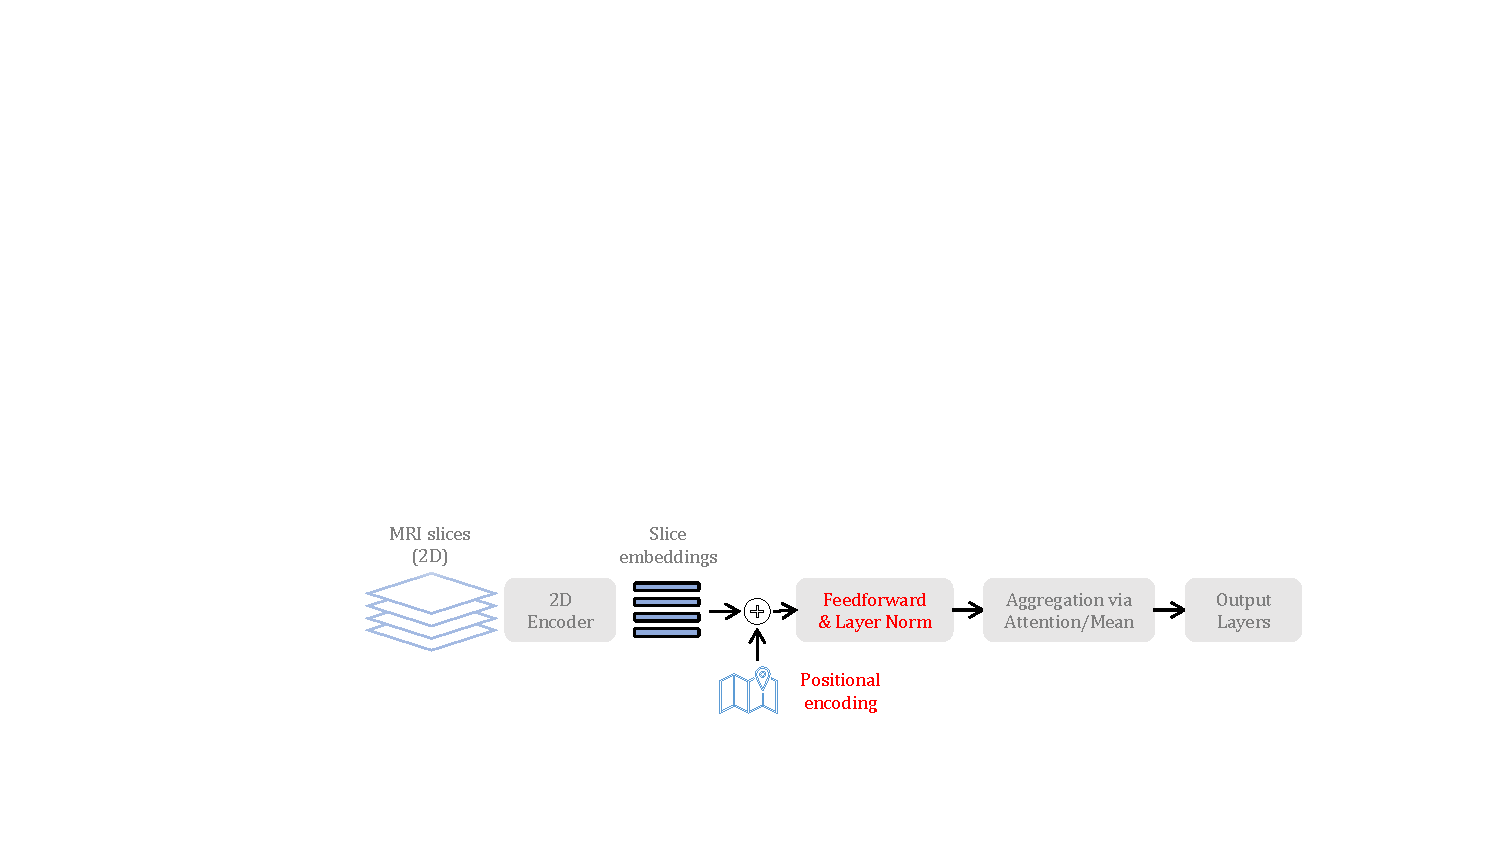
\includegraphics[width=0.85\textwidth, trim={6cm 2.2cm 3cm 8.9cm},clip]{figures/arch-diagram-med-neurips.pdf}}
    \caption{Positional encoding in the 2D-Slice-CNN architecture. Newer  components (compared to~\cite{gupta2021improved}) are shown in red font.}
    \label{fig:approach}
\end{figure*}

The go-to approach to train models that take raw 3D MRIs as input is to use 3D convolutional layers
(e.g.,~\cite{peng2019accurate, hu2020brain, guanLearning2021}).
Instead,~\cite{gupta2021improved} used 2D-CNNs to encode individual slices and combined the slice representations with permutation-invariant operations such as mean or attention. Compared to 3D-CNNs, these 2D-Slice-based models tend to be less accurate as they may lose spatial information due to permutation invariance. To this end, we encode positional information in the model by introducing positional encodings similar to transformers~\cite{vaswani2017attention,dosovitskiy2021image}. In particular, these are added to the slices' representations and trained end-to-end with other model parameters (see Fig.~\ref{fig:approach}). Suppose the MRI consists of $K$ 2D slices ($x_k, k \in \{1\ldots K\}$) that are each embedded to a d-dimensional representation, $r(x_k)$ with the 2D slice encoder. The model will compute $r(x_k)+p_k$, where $p_k \in \mathbb R^d$ is a trainable vector and depends only on $k$. Fixed positional encodings can also be used. However, this work considers positional encodings as trainable.





Further, motivated by the transformer architecture, we also added a feed-forward layer and layer norm after the attention (i.e., for attention-based aggregation) as that improved the performance on brain age prediction slightly (2.86 reported in~\cite{gupta2021improved} vs.\ 2.83 MAE in our case).












